\documentclass[12pt]{article}
\usepackage[utf8]{inputenc}
\usepackage{geometry}
 \geometry{
 a4paper,
 total={170mm,257mm},
 top=2.54cm, bottom=2.54cm, left=3.18cm, right=3.18cm
 }
 \usepackage{graphicx}
 \usepackage{titling}
 \usepackage{indentfirst}

 \usepackage{fontspec}
% 设置正文字体
\setmainfont{Times New Roman}

\usepackage{setspace}
\usepackage{hyperref}

 \title{Feature Generation from Text Collections using TFIDF Representation
}
\author{name}
\date{November 2024}
 
 \usepackage{fancyhdr}
\fancypagestyle{plain}{%  the preset of fancyhdr 
    \fancyhf{} % clear all header and footer fields
    \fancyfoot[C]{\thepage}
    % \fancyfoot[L]{\thedate}
    \fancyhead[L]{Feature Generation}
    \fancyhead[R]{\thedate}
}

\makeatletter
\def\@maketitle{%
  \newpage
  \null
  \vskip 1em%
  \begin{center}%
  \let \footnote \thanks
    {\LARGE \@title \par}%
    \vskip 1em%
    %{\large \@date}%
  \end{center}%
  \par
  \vskip 1em}
\makeatother

% \usepackage{cmbright}

\begin{document}

\maketitle

\noindent\textit{\begin{tabular}{@{}ll}
    Student & \theauthor\\
    ID & 123 \\
    Course & course name\\
\end{tabular}}

\setlength{\baselineskip}{20pt}
\setlength{\parskip}{1ex}

\section{Preprocessing}
\subsection{Read and Split}
Reading datasets from files and directories is the basic work of the text categorization task. The datasets used in this experiment are stored in five subdirectories, where the names of the subdirectories correspond to the tag names, and the files in the subdirectories are text files of the corresponding categories. For the sake of possible subsequent categorization tasks, both text content and labels should be loaded at the same time when loading. So, I use \textbf{list} to store the text data and labels in this step, and also use a \textbf{dict} type to store the mapping from labeled text to values. The values corresponding to the labels are simply noted as their index order.

Firstly, use \textbf{os.listdir()} to get all the subfolders and labels:
\begin{figure}[h]  % 'h'表示在这里插入
    \centering     % 使图片居中
    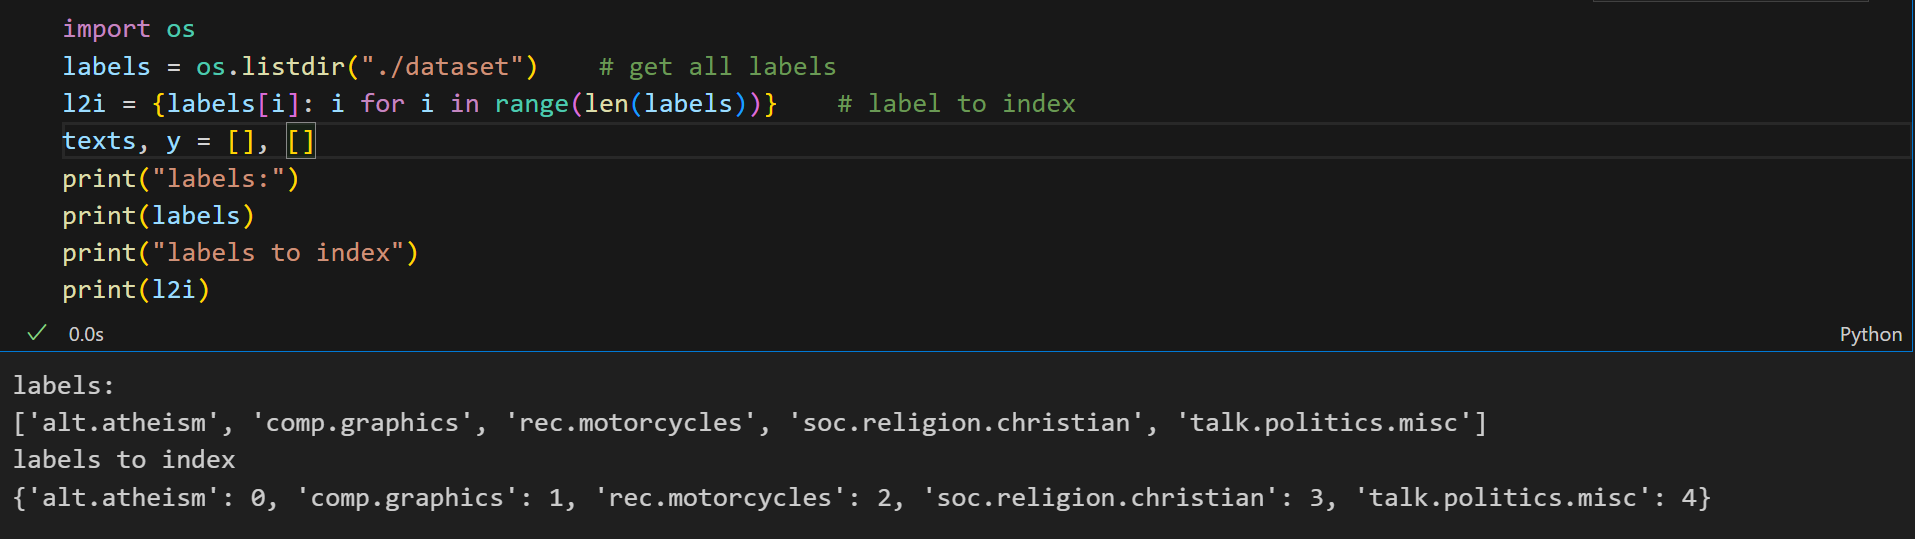
\includegraphics[width=0.8\textwidth]{images/image1.png}  % 设置图片宽度,image_filename是图片文件名
    \caption{load labels}  % 图片标题
    \label{fig:image1.1}  % 为图片设置标签,以便引用
\end{figure}

As shown in Figure \ref{fig:image1.1}, I got all the labels successfully in this step.

Next, for each label, use \textbf{os.listdir} separately to get all the files contained in the subdirectory and use \textbf{codecs.open()} to read the text content. For garbled raw text, I use \textbf{str.split()} to split it into individual words.

\begin{figure}[h]  % 'h'表示在这里插入
    \centering     % 使图片居中
    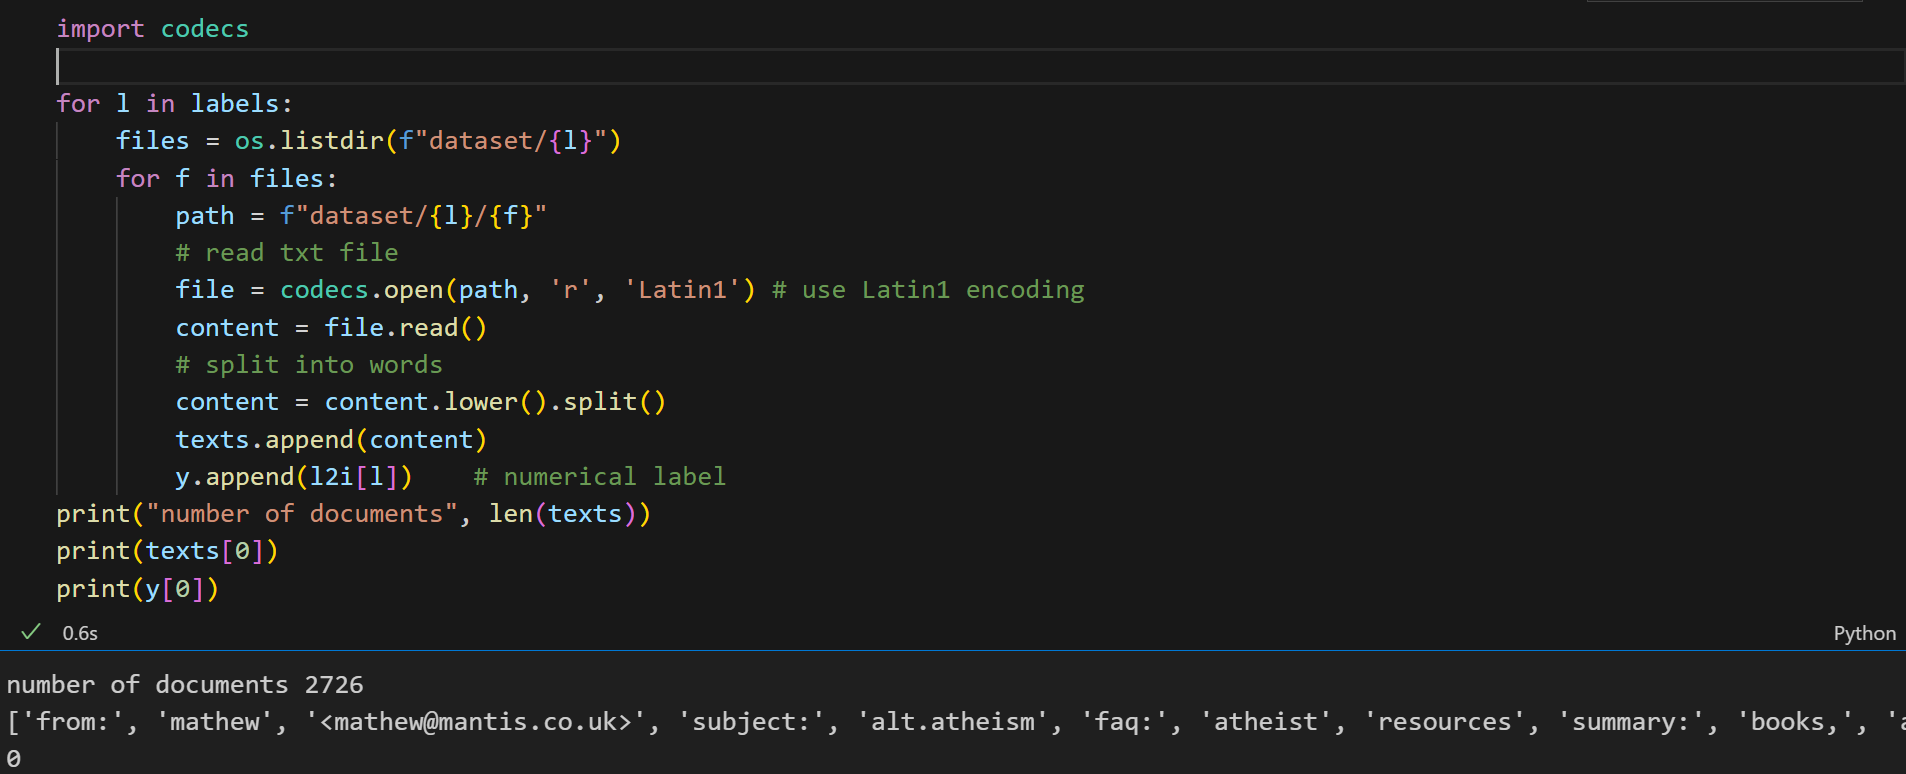
\includegraphics[width=0.8\textwidth]{images/image2.png}  % 设置图片宽度,image_filename是图片文件名
    \caption{load texts}  % 图片标题
    \label{fig:image1.2}  % 为图片设置标签,以便引用
\end{figure}

As shown in Figure \ref{fig:image1.2}, I managed to load all the text files under the labels, and each document was converted into a list containing one single word. In this step, I also loaded the corresponding numeric labels \textit{y}. 


\subsection{Remove Stopwords}
In this step, I use \textbf{re.sub()} to remove non alphabetical characters in a regular expression matching pattern. In this way, each document is given a list consisting entirely of words.The next step is to remove stopwords in the sentence that have little or no point of use in conveying the meaning. In this experiment, the stopwords have been given in a txt file. Notice that this step involves a lot of looking up whether a word appears in the list of stopwords or not. Therefore, I converted the stopwords to the type \textbf{set}, a hash-table based data structure that enables efficient data lookups.

\begin{figure}[h]  % 'h'表示在这里插入
    \centering     % 使图片居中
    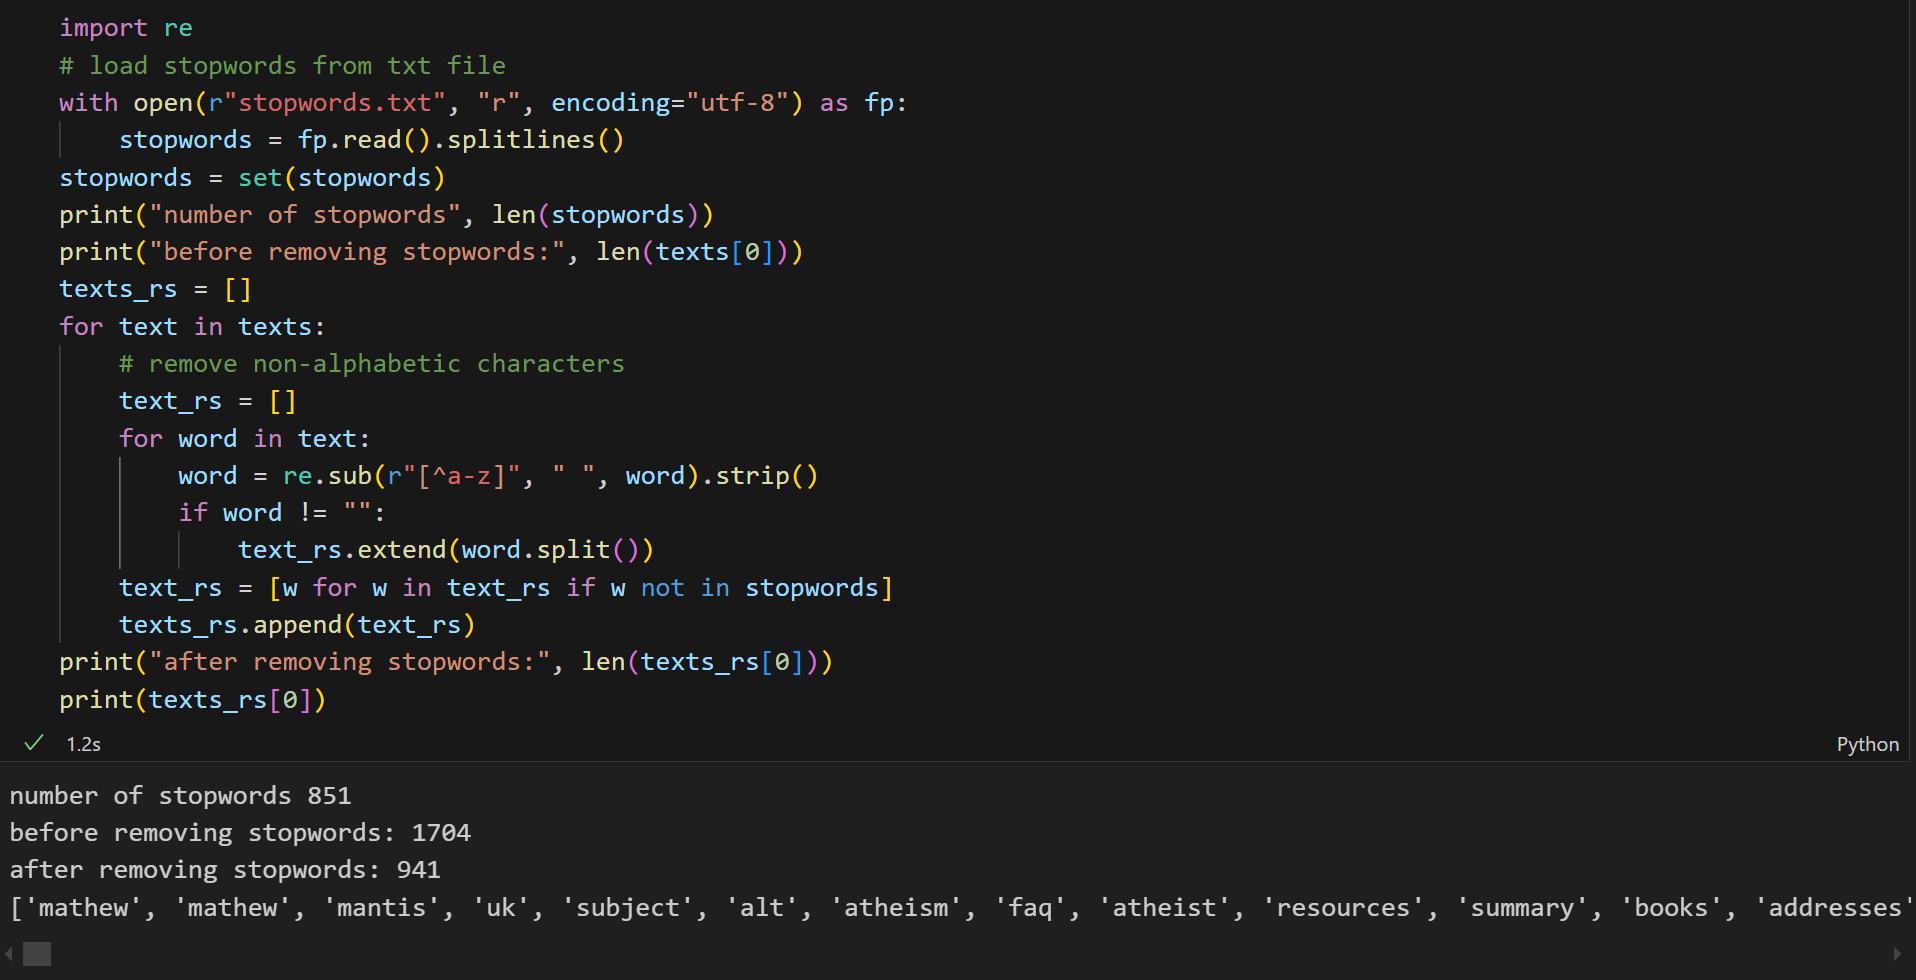
\includegraphics[width=0.8\textwidth]{images/image3.png}  % 设置图片宽度,image_filename是图片文件名
    \caption{remove stopwords}  % 图片标题
    \label{fig:image1.3}  % 为图片设置标签,以便引用
\end{figure}

When deleting a non-alphabetical character from a word, I initially delete the character directly. However, I find this often turns the part into a longer meaningless word, such as [Alt.Atheism], which becomes [altatheism]. It would be more sensible to separate the words before and after the non-alphabetical characters, which would result in two words: [alt atheism].

As can be seen from the results, the number of stopwords is 851. After this step, the number of words contained in the first document in the dataset decreases from 1704 to 941. 

\subsection{Word Stemming}
The goal of word stemming is to simplify the words to their basic forms, including removing the tense changes of verbs, plural forms of nouns, etc. I implemented this with the help of \textbf{SnowballStemmer} from the nltk library\cite{nltk}.

\begin{figure}[h]  % 'h'表示在这里插入
    \centering     % 使图片居中
    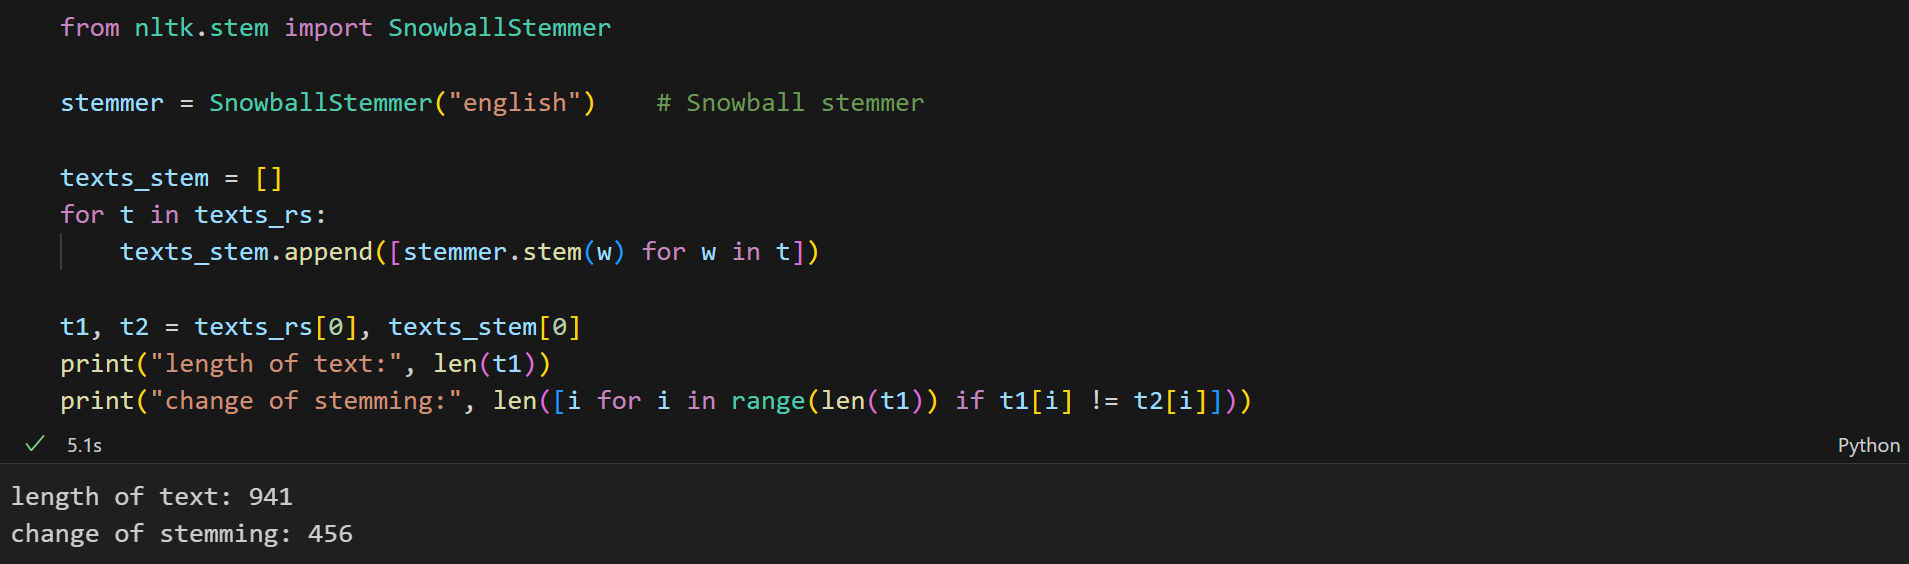
\includegraphics[width=0.8\textwidth]{images/image4.png}  % 设置图片宽度,image_filename是图片文件名
    \caption{word stemming}  % 图片标题
    \label{fig:image1.4}  % 为图片设置标签,以便引用
\end{figure}

In Figure \ref{fig:image1.4}, for a document of length 941, the stemming step changed 456 of the words.

\section{TFIDF Representation}
To achieve better code compactness and readability, I encapsulated the TFIDF word vectorization functionality into a single class. This class takes as input the list of document words preprocessed in the previous step and outputs the document-by-word matrix.

The main properties of this class are defined as follows:
\begin{itemize}
    \item \textit{document\_freq}: (dict), represents the number of document occurrences of the word in the dataset.
    \item \textit{vocab\_table}: (dict), denotes the index of the word in the second dimension of the document-by-word matrix.
    \item \textit{num\_docs}: (int), number of documents in the dataset.
    \item \textit{dims}: (int), total number of words in the dataset
\end{itemize}

Getting the above information from the dataset before formally calculating tfidf will greatly facilitate subsequent calculations.

\begin{figure}[h]  % 'h'表示在这里插入
    \centering     % 使图片居中
    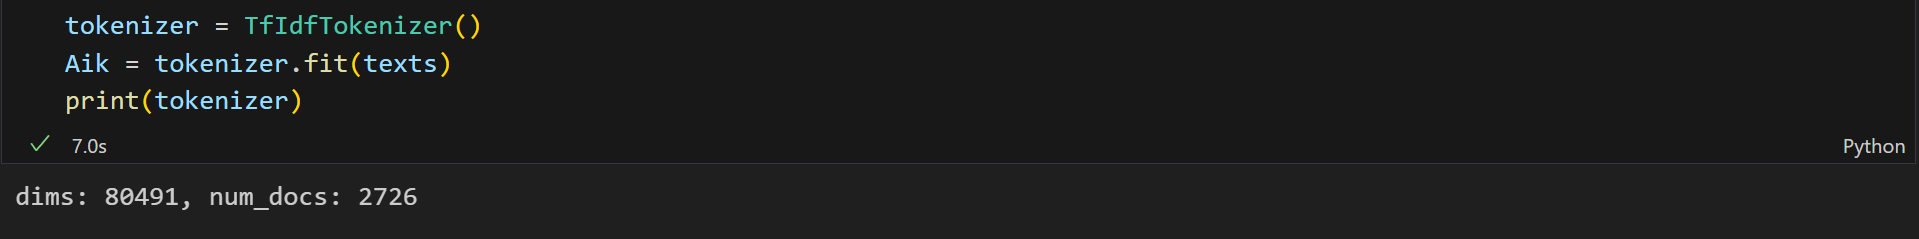
\includegraphics[width=0.8\textwidth]{images/image5.png}
    \caption{class attributes}  % 图片标题
    \label{fig:image1.5}  % 为图片设置标签,以便引用
\end{figure}

As shown in Figure \ref{fig:image1.5}, the dataset contains 2726 documents, with a total of 80,491 different words. The \textit{vocab\_table} contains a mapping of each word to a numeric index.
    
\subsection{Word Frequency}
When calculating the frequency, I processed each document individually, counting the occurrences of each word. 
This is done by initializing a zero-filled array with dimensions [number of documents, number of unique words]. 
Then, for each word in each document, I find the index in the vocab\_table and increment the corresponding position in the array. 
After the traversal is completed, this array is accumulated in the second dimension to obtain the total number of words in each document, and the total number is used to calculate the frequency.

\begin{figure}[h]  % 'h'表示在这里插入
    \centering     % 使图片居中
    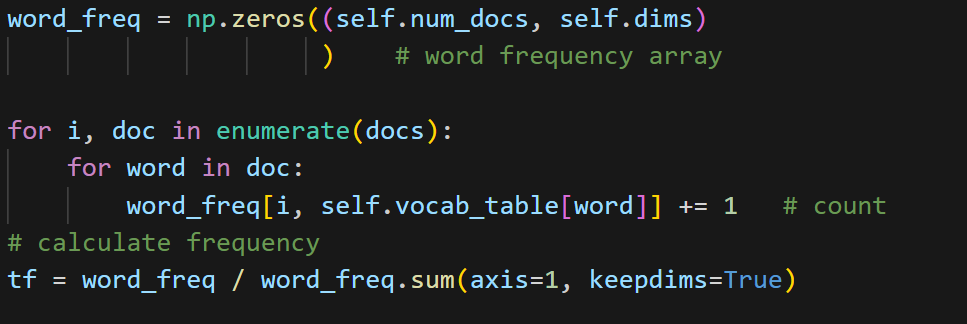
\includegraphics[width=0.8\textwidth]{images/image6.png}
    \caption{word frequency}  % 图片标题
    \label{fig:image1.6}  % 为图片设置标签,以便引用
\end{figure}

\subsection{Document Frequency}
In this step, I obtained the document frequency of each word in the dataset. 
 This information is represented via a dict with key as word and value as number of times. For each word in each document, if it is not in the dict, add it to the dict and initialize the count to 1; conversely, the count is incremented by 1.

\begin{figure}[h]  % 'h'表示在这里插入
    \centering     % 使图片居中
    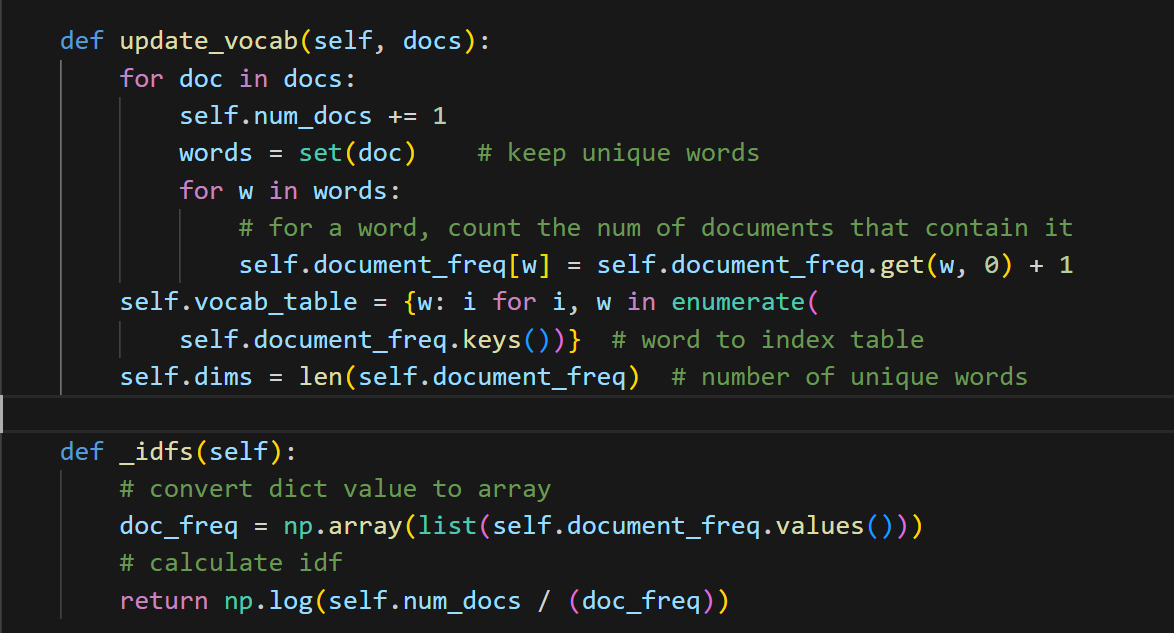
\includegraphics[width=0.8\textwidth]{images/image7.png}
    \caption{document frequency}  % 图片标题
    \label{fig:image1.7}  % 为图片设置标签,以便引用
\end{figure}

\subsection{Normalize}
TF-IDF is calculated using formula \ref{eqn:1}:
\begin{equation}
    a_{ik} = log(f_{ik}+1.0) * log(\frac{N}{n_k})
    \label{eqn:1}
\end{equation}

I used the array representation in numpy when calculating tf and idf, so there is no need to calculate element by element in this step, just multiply directly using the \textbf{broadcast} mechanism in numpy.

In regularization process, I use numpy to get the sum of squares of the elements in each row of the array and broadcast the division to each element. 
\begin{figure}[h]  % 'h'表示在这里插入
    \centering     % 使图片居中
    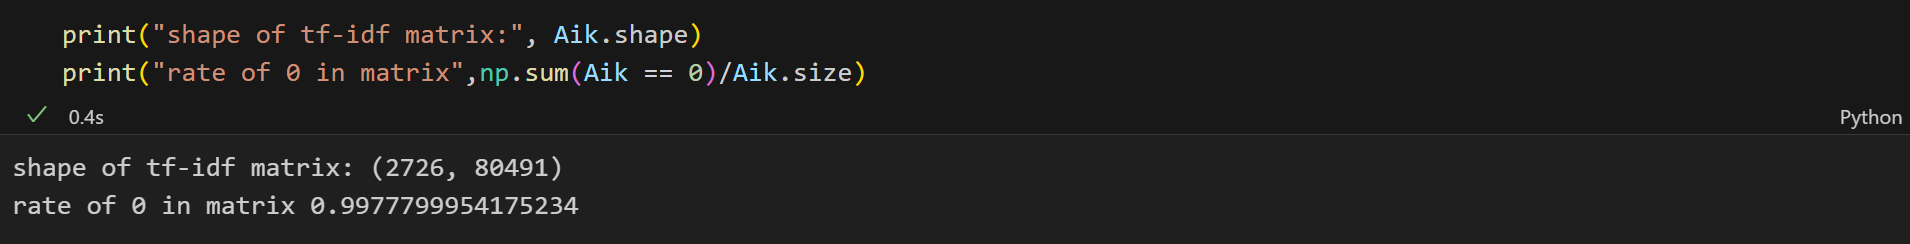
\includegraphics[width=0.8\textwidth]{images/image8.png}
    \caption{TF-IDF result}  % 图片标题
    \label{fig:image1.8}  % 为图片设置标签,以便引用
\end{figure}

The results obtained are shown in Figure \ref{fig:image1.8}. Two things are worth noting: 
\begin{enumerate}
    \item the result is quite \textbf{high-dimensional}, with a matrix of the shape (2726, 80491)
    \item the result is highly \textbf{sparse}, with up to 99\% of the transformed word vector matrix is 0
\end{enumerate}

The reason for these two occurrences may be caused by using all the words in the dataset, which can lead to unnecessary storage and computational consumption. Therefore, I tried to remove the low-frequency words from the dataset and encode using only some of the high-frequency words. The way to implement this is to build a new class by inheriting the previous class, rewrite some methods, count the word frequencies in the statistics set, and encode only the 5000 words with the highest frequency.

\begin{figure}[h]  % 'h'表示在这里插入
    \centering     % 使图片居中
    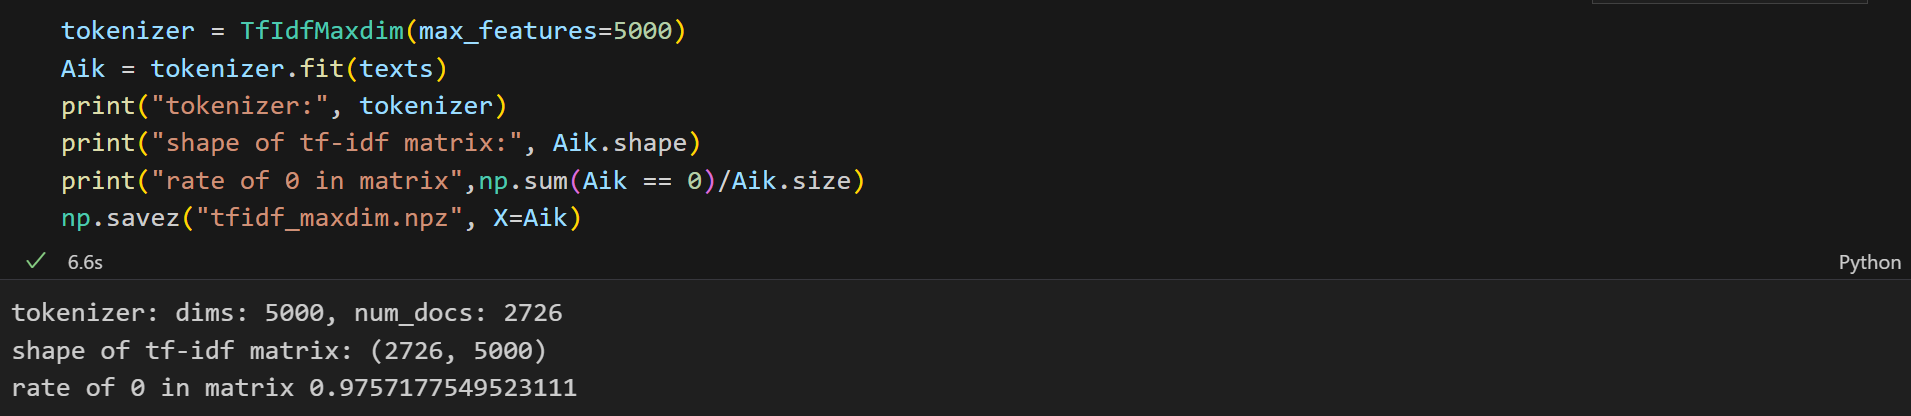
\includegraphics[width=0.8\textwidth]{images/image9.png}
    \caption{limited dimensions}  % 图片标题
    \label{fig:image1.9}  % 为图片设置标签,以便引用
\end{figure}

The results of word vectorization after limiting the dimensionality are shown in Figure \ref{fig:image1.9}, where the second dimension of the word matrix is reduced from 80,491 to 5,000, and the ratio of 0 in the result is reduced to 97\%. I also observed that \textbf{the size of the npz file} obtained by the original method is as large as 1.5GB, and the npz result after restricting the dimensionality is only about 100MB.

\section{Conclusion}
Text vectorization is the groundwork for various Natural Language Processing (NLP) tasks, including text categorization. In this experiment, I inplemented the popular TF-IDF(Term Frequency-Inverse Document Frequency)  vectorization method and successfully converted the ONE dataset into a word vector matrix. By calculating the word frequencies within documents and document frequencies across the corpus, TF-IDF achieves straightforward and efficient word vectorization.
The result is a highly sparse matrix, which effectively captures the relative importance of words in the dataset.
During this experiment, I observed that utilizing the entire vocabulary of the dataset for TF-IDF tends to bring about high memory consumption, which can be alleviated by using a subset of high-frequency words.

\bibliographystyle{unsrt}
\bibliography{refer.bib}

\end{document}
